\chapter{Discussion}
\label{chap:discussion}





With the disks now fit, we may interpret our results. Since this project was based around the question of how environment influences protoplanetary disks, we would like to compare our best fit values to other disks, including to one other from the ONC \citep{Factor2017} as well as to others outside of it. We begin with a brief review of the relevant literature on the three disk profiles that we fit (density, temperature, and chemical) so that we may frame our results in a meanigful context.

% REWORK: I think somewhere before this section, ideally right at the start of the chapter, you should lay out a bunch of caveats about our abundances — particularly that they are derived from the MAJOR assumption the total disk gas mass will be 100x the dust mass derived from continuum emission.  It needs to be in everyone’s mind while they are reading about the modeling.  



\section{Reflections on the Fits}

As discussed in \S\ref{subsection:co_fit}, our attempts to fit the CO line were overwhelmed by the significant cloud contamination around the disk, resulting in physically-unreasonable best-fit values. If this run had converged to physical values, we would have used its disk mass results in the other runs, but since these results are not to be trusted, we instead continued to use the disks' mass values presented in \citet{Williams2014}, which were inferred from continuum emission.

% REWORK: be quantitative about "decidedly"
% REWORK all percentages: I’m not really interested in what percentage agreement is reached, but rather the significance of that agreement.  Do they agree to within 1-sigma, for example?  All of these percentage values need to be rewritten in terms of significance.
% The 50% figure is a little more interesting, but here I might just insert the actual values.  Something like: “The best-fit atmospheric temperature for HCO+ (xxx+/-xxx K) is significantly higher/lower than the corresponding value for HCN (xxx+/-xxx K), but this is at least somewhat expected…”
The \hco and HCN runs converged into impressive agreement, although the posteriors from the \hco line show smaller uncertainties than those of the HCN line. Both the \hco and HCN lines show molecular abundances in disk A that are almost two orders of magnitude than those in disk B (discussed later). The two lines' fits for disk A's outer radius agree to within around 1\% (although the HCN fit is significantly less certain than the \hco fit) and the lines' best-fit $q$ values agree to within 15\%. Atmospheric temperatures for disk A in both lines are large and significantly different, with the \hco line preferring a temperature 50\% greater than HCN's, but this is at least somewhat expected, as the two molecules are emitting from different regions of the disk and thus could reflect different regions of its temperature profile. In both lines, disk A's temperature structure power law index, $q$, is decidedly positive, although we expect this parameter to not settle with absolute certainty on a single value, since the observations don't have enough spatial resolution to constrain it tightly.


% REWORK: What does 'expected' mean? Useful?
Fits for disk B are systematically less well constrained, primarily in outer radius. This likely reflects the fact that it is smaller, unresolved, and more easily overrun by emission from features that were not modeled, such as cloud contamination, excess disk A emission, and emitting material shared by the two disks. The outer radius was most notably affected by these features, yielding somewhat bimodal posteriors in both \hco and HCN as the walkers sometimes tried to fit the outer features. As discussed in \S\ref{subsection:hcn_fit}, a posteriori cuts of the HCN model's MCMC chain limiting disk B's outer radius to $\geq$220 au - effectively manually choosing one of the posterior's two modes -  changed the best-fit parameters significantly, most notably leading the HCN fit's value for disk B's outer radius into agreement with \hco. It also pushed disk A's HCN abundance more than a full order of magnitude higher, and into nearly perfect agreement with results from HCN fitting in \citet{Factor2017}. Whether this is a reasonable thing to do is not clear to me.






\section{Physical Structure}
% - Start off comparing basic stuff like masses and radii of your disks, so that we get the idea that relative to large populations of disks they are big and dense, but that relative to Sam’s disk they are comparable in mass/radius.

% REWORK: I’m not sure this is the study you want to talk about here, or how you want to present it.  A couple of thoughts:
% - You start off comparing the disks’ masses and radii to other disks in Orion, which is great.  Clearly apples to apples.
% - Next, you want to compare your disks to disks in low-mass SF regions.  Also great.  But to discuss how the properties of your disks compare to the properties of disks in low-mass SF regions, you need to compare the same data.  So you’d want to look for a study (and there are lots! some of which you talk about below!) that compiled disk masses based on mm continuum measurements, assuming 100:1 gas:dust mass ratio like Rita did.
% - The study you’re referencing here (Miotello2016) is really great and important!  But I think you want to discuss it in the context of the assumptions you made and why they might not be correct.  Specifically, this study provides evidence that 100:1 may not be a valid assumption for the gas:dust mass ratio in protoplanetary disks.
% So, all good stuff, but just organized weirdly.  I think you should also describe a bit more of the methodology of how the authors “analyze several CO isotopologues” — this is a nonstandard (but very interesting!) method that involves comparison of data with radiative transfer models of a large grid of generic disk models, so you should say a bit more about what they did so that your reader can better interpret it.  

% REWORK: One thing you need to make sure to include in any discussion of disk mass ranges is a discussion of sensitivity limitations.  Are there disks with masses less than 1 M_Jup?  Probably!  Are they detectable?  Nope.  Also, the sensitivity limits are lower for low-mass SF regions than for high-mass, simply because they’re closer, which is another important caveat that is currently missing from your discussion. 



To get a sense of how these disks' physical characteristics (i.e. mass and radius) compare to other protoplanetary disks, it is useful to compare our results to other disks in the Orion Nebula Cluster, as well as others in low-mass star forming regions (SFRs). It is worth again reiterating that many of the reported disk gas masses in the literature \citep[as well as the one we use here from ][]{Williams2014} are calculated from continuum emission (which traces dust mass), and then scaled by the factor of 100 to return a gas mass. However, as briefly discussed in \S\ref{chap:introduction}), this ISM-based gas/dust ratio has been shown to be neither constant across disks nor best approximated by 100:1.


\citet{Williams2014} presented a method infer a disk's gas mass while avoiding the use of the 100:1 gas/dust ratio in their calculations by comparing ratios of CO isotopologues. The method they present involves developing parametric disk models over a wide range of parameters (similar to the modeling process used in this study), calculating the resulting emission intensities of selected lines (generally C$^{18}$O and $^{13}$CO due to their relative abundances but lack of cloud-induced contamination), holding certain molecular and atomic abundance ratios fixed (most notably, their CO/H$_2$ ratio is held constant at the molecular cloud-level of 10$^{-4}$) and then inferring the mass of an observed disk by locating where it falls on that grid of models. Their application of the method to nine well-studied disks in Taurus yielded masses appreciably lower than the use of a 100:1 gas/dust ratio would have implied, instead returning a wide range of ratios that were centered around 10:1. Analysis of a survey of 89 disks in Lupus \citep{Ansdell2016} using this method showed a similar trend, although due to insufficient C$^{18}$O detections, only 11 of the disks were able to be fully estimated; another 25 had upper limits places on their gas masses.

In \citet{Miotello2014,Miotello2016}, the authors build on the methods of \citet{Williams2014}, using CO isotopologue ratios to find gas mass, but avoid the use of fixed abundance ratios by integrating a full chemical-reaction network to reflect the effects of freeze-out and photodissociation (the two main effects driving chemical evolution). This allowed them to expand the sample of constrained gas masses from the \citet{Ansdell2016} survey from 11 to 34. Their results again show that the use of a fixed gas/dust ratio is inappropriate.


% REWORK: Maybe good to include discussion of Ansdell2017? Survey of 92 disks in sigOri, only 6 CO detections, use a comb of Williams and Best/Miotello methods.

\begin{figure}[h]
  \hspace*{\fill}%
  \subcaptionbox{}{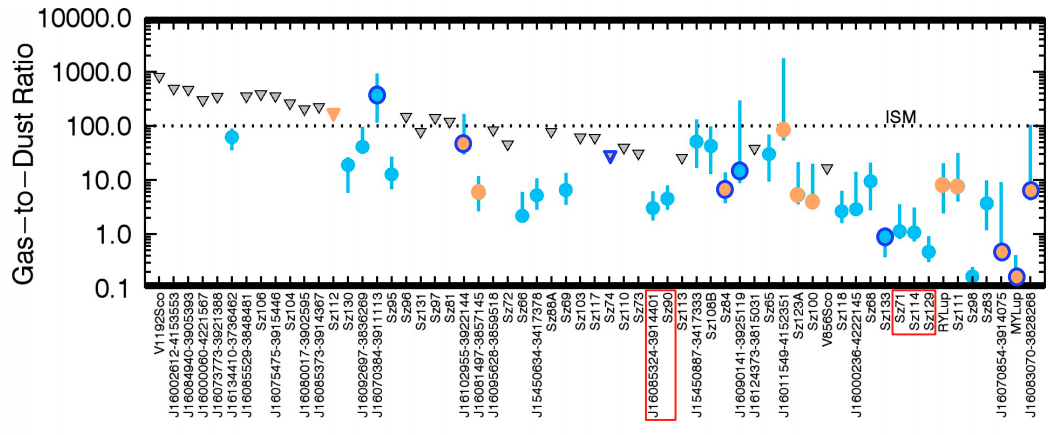
\includegraphics[width=0.5\linewidth]{Miotello17_GDRs.png}}%
  \subcaptionbox{}{\includegraphics[width=0.5\linewidth]{Miotello17_GDR_ratios.png}}%
  \hspace*{\fill}%
  \caption{blah balh}
  \label{fig:GDRs}
\end{figure}


With this in mind, the values we use for the masses of disk A and disk B are 0.075 M$_\odot$ and 0.029 M$_\odot$ (78.66 and 29.88 Jovian masses), respectively, drawn from \citet{Williams2014}. Our best-fit radii from the \hco fits were around 340 and 148 au, respectively.



% REWORK: Maybe add a sensitivity limit.
% REWORK: percentages to sigmas
In the survey of ONC proplyds that originally provided these data, \citet{Mann2014} inferred total disk masses and fit the disks with 2D elliptical Gaussians, and using the resulting semi-minor and -major axes of the disks as approximate measures of the disks' radial extents. Disk A in the present system was, by their measure, the most massive disk in the study, 75\% ($37\sigma$) more massive than the study's next most massive disk, d216-0939 \citet[which was the subject of][]{Factor2017}; disk B was the fifth most massive. Disk A had the study's fourth largest semi-major axis\footnote{The authors' measurement of disk A's semi-major axis, at 268 au, is $2.6\sigma$ smaller than our fit measurements. The survey's reported semi-major axis for d216-0939 was also smaller than the fit value in \citet{Factor2017}, though by less than $1\sigma$.}. The authors did not fit disk B's radial extent; however, our measurement of 145 AU would make it the eleventh (out of 22) largest disk in the survey. Thus, disk A is on the very high end of the study's mass and radius range, while disk B is apparently quite dense and of median radial extent.




\citet{Eisner2018} conducted a particularly comprehensive survey of 104 detected disks in the heart of M42 within 0.14 pc of $\theta^1$ Ori C, measuring the disks' dust masses (from continuum flux) and radii (from the half-max half-width of the major axis of 2D Gaussian fits to the disks), and comparing their results to similar measurements from other surveys of disks in low mass SFRs. These comparisons are summarized in fig.\ref{fig:eisner18_disk_properties}, showing the distributions of masses and radii of disks in each survey. From them, we see that these M42 disks are characteristically denser and radially truncated, as shown by the ONC track's relatively high position on the mass plot and relatively low position on the radius plot. By inferring the dust masses of the present binary's disks using the 100:1 gas/dust ratio (yielding masses of around 250 M$_\oplus$ and 95 M$_\oplus$ for disk A and B, respectively) and recalling our fit radii (around 340 and 148 au, respectively), we may place these two disks on these plots and find that they are far more massive than the M42 disks and that disk A is more massive than any of the disks in all the surveys. However, while the ONC disks in this plot exhibit an atypically high density (the highest-mass disks have mass/radius ratios of around 1.5 M$_\oplus$/au) relative to the other survey's disks (which are closer to of order 0.5 M$_\oplus$/au), disk A and B land at 0.75 and 0.65, respectively. This indicates that, while they are still somewhat more dense than the disks from low-mass SFRs, they show neither the radial truncation nor high densities found in the M42 disks.



\begin{figure}[h!]
  \centering
    \hspace*{\fill}%
    \subcaptionbox{Disk mass distribution across surveys}{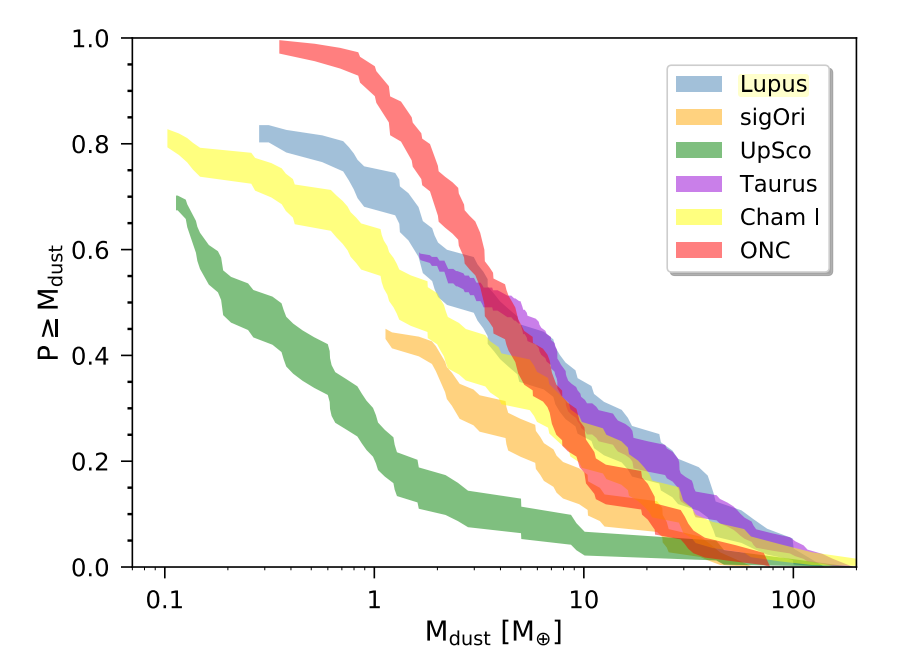
\includegraphics[width=0.5\linewidth]{dust_mass_dist_Eisner18.png}}%
    \subcaptionbox{Disk radius distribution across surveys}{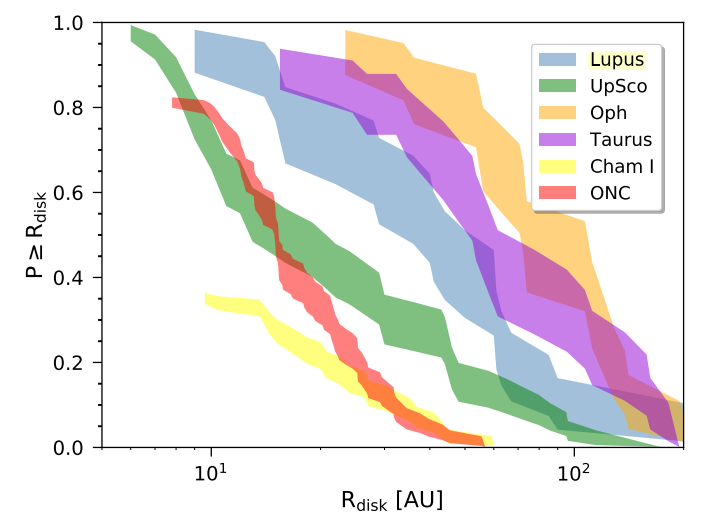
\includegraphics[width=0.5\linewidth]{dust_radius_dist_Eisner18.png}}%
    \hspace*{\fill}%
    \caption{Plots of disk masses and radii frequencies \citep{Eisner2018}. Blah blah blah}
    \label{fig:eisner18_disk_properties}
\end{figure}




\citet{Williams2019} surveyed 279 disks in $\rho$ Ophiuchus and found some stuff from dust emission. Probably good to screengrab some of their plots

The resulting gas masses from \citet{Miotello2017} ranged from $10^{-6}$ to $10^{-3}$ M$_\odot$, with the most massive at 1.5 $\times 10^{-3}$ M$_\odot$ (1.6 Jovian masses). Since the disks were not spatially resolved, radii were not measured, so no comparison of their compactness can be made.

\citet{Ansdell2016} and \citet{Ansdell2018} characterized the mass (both dust and gas) and radius distributions of protoplanetary disks in Lupus using CO isotopologues and continuum emission. Of these gas masses that they were able to constrain, they found disks to range from around 1-10 Jovian masses.


% These results indicate that the disks that are the subject of this study are atypically massive (and maybe wide)




\subsection{Comparison to Binaries}

% T Tauri Binary surveys: Duchene1999, Kraus2008, Kraus2011

% Binaries in the ONC (2012) (not radio): https://www.aanda.org/articles/aa/pdf/2012/04/aa18314-11.pdf
% Binaries in Taurus (2012): Harris2012
% Binaries in Taurus (2019): Akeson2019
% Binaries in rho Ophiucus (2014): Akeson2014 (49 systems, 63 stars)
% Binaries in rho Ophiucus (2017): cox2017
% GG Tau A: Dutrey2014
% In close (\textless100 au) binary systems, it is predicted \citep{someone} that circumstellar disks should develop around each star in addition to an outer circumbinary disk. \citet{Dutrey2014} used high-resolution ALMA observations to reveal such a system around a heirarchical triple system (where a binary pair is one element of a larger binary) revealed complex interactions between the various disks. However, since both tiers of this system are very close (the outer binary has an apparent separation of 35 au, while the inner pair are separated by just 4.5 au), the system is not entirely comparable to our present binary.

% V2434 Ori: 05 35 25.23 -05 15 35.69

% Distance to Theta Ori C
% Theta Ori C: 05 35 31.43 -05 25 16.36
% sqrt(6.2^2 + (10*60 -9)^2)

% Nu Ori: 05 35 31.36	-05 16 02.58
% sqrt(6.1^2 + (1*60 -32)^2) = 11147au = 0.05pc


We must also consider the fact that our disks are in a binary. While this work is not meant to be a complete review of multiple star systems \citep[the interested reader is referred to ][for a more comprehensive review]{Duchene2013}, some review of the relevant literature is warranted to frame our interpretation of the present system.

Binaries (and higher-order systems, which generally form as heirarchical pairs) are quite common, with around 30\% of low- and intermediate mass Main Sequence stars presenting with companions; that number climbs to 70\% for high mass stars\citep{Sana2012}, and surveys of younger, T Tauri stars in low-mass regions show even higher fractions, often doubled, up to almost 80\% in Taurus \citep{Kraus2011}, for example. However, regions of higher densities, like the ONC, seem to have the opposite effect, as \citet{Reipurth2007} found that the 781 sources within 60'' of $\theta$ Ori C contained only 78 multiple systems (with apparent separations between 67 and 675 au), yielding to a companion fraction of just 9\%. There is notable subsetting within that population, particularly with a defiency of wide ($0.''5 < a < 1.''5$, or around 200-600 au at the ONC's Gaia-measured distance of 389 pc) binaries closer to $\theta_1$ Ori C (see Fig.\ref{onc_binary_stats}). At a distance of around 591'' from $\theta_1$ Ori C, our binary is far enough away from $\theta_1$ Ori C that, based on Fig.\ref{onc_binary_stats}, it is not an unexpected binary to find. Additionally, with an angular separation of 1.''1, it is represents one of the wider pairs in the ONC.


\begin{figure}[h]
  \hspace*{\fill}%
  \subcaptionbox{}{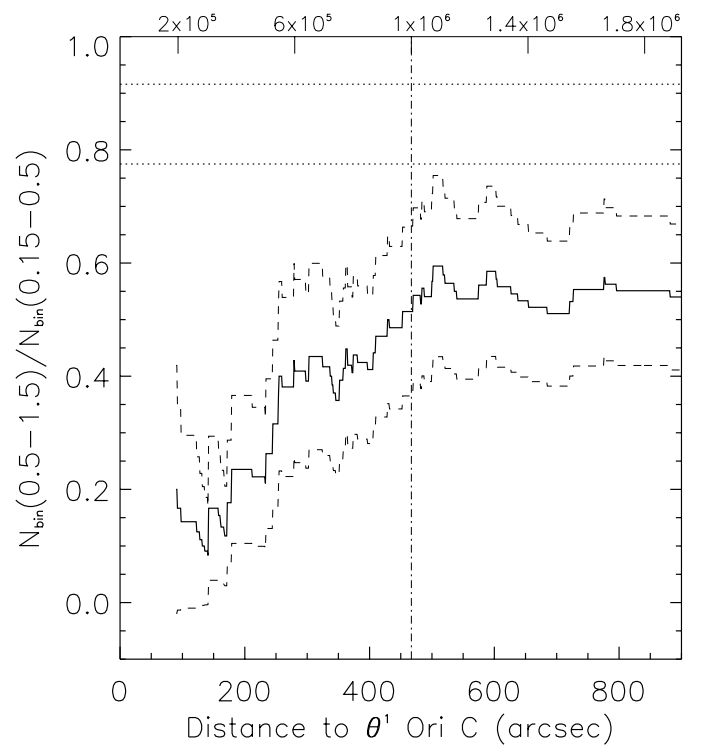
\includegraphics[width=0.5\linewidth]{Reipurth2007_binfrac_by_dist_thetaoric.png}}%
  \subcaptionbox{}{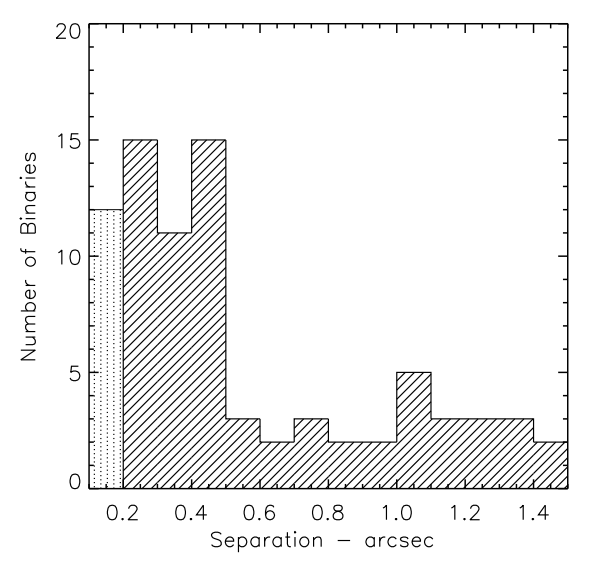
\includegraphics[width=0.5\linewidth]{Reipurth2007_binfreq_by_sep.png}}%
  \hspace*{\fill}%
  \caption{Statistics for binary pairs in the Orion Nebula Cluster \citep{Reipurth2007}. The present system is around 591'' from $\theta_1$ Ori C, putting it beyond the radius apparently affected by the massive star.}
  \label{fig:onc_binary_stats}
\end{figure}



% REWORK: Add stuff about binary formation.
% There are two favored pathways to the formation of multiple star systems: the fragmentation of a gravitationally unstable disk \citep[e.g. ][]{Kratter2010} and turbulent fragmentation of the molecular cloud \citep{Offner2010}. Of these two pathways, it has seemed that
% A survey of 17 multiple protostar systems in Perseus with separations less than 600 au by \citet{Tobin2018} implied that disk fragmentation, rather than REWORK, is likely the dominant formation method for binary systems.

Less is known about disks in binary systems than the stars themselves. Several millimeter surveys have observed a number of disks in binary systems in various regions, most notably in Taurus and $\rho$ Ophiucus. Since these regions are low-mass SFRs, they are qualitatively different environments than the ONC, but provide us with a good starting point to compare to.

% Not sure how to slide this in. 'It has long been known \citep[and references contained therein][]{Jensen1995} that close (\textless50-100 au) binaries have lower combined millimeter fluxes than wider binaries or single stars.'

\citet{Harris2012} observed 23 multiple-star systems in Taurus using the Submillimeter Array. In it, they found a strong anticorrelation between system brightness and projected separation between components, with wide pairs (\textgreater300 au) showing similar brightness to that of two single stars, while tight pairs (\textless30 au) suffer a $5\times$ decrease from the equivalent sum of individual brightnesses (although the presence of circumbinary disks around binaries of any separation make the system significantly brighter; see Fig.\ref{fig:harris2012_binary_brightnesses}).

\citet{Akeson2019} built on these results with an ALMA survey of additional binaries in Taurus, developing a sample of 151 sources with resolved millimeter detections, 99 of which were in binary systems\footnote{The fact that this number is odd just reflects that at least one of the binaries had an undetected secondary member.}. From this sample, they found that disks around the binaries' primary (more massive) star contributes, on average, 62\% of the disks' total combined mass, although this distribution has a wide spread. They also developed the observation by \citet{Harris2012} \citep[and, previously, ][]{Jensen1995} that tighter binaries led to lower fluxes, finding that, as a function of stellar mass, disks in binaries have systematically lower masses than their isolated counterparts, and that this mass truncation is more apparent in tighter binaries (see Fig.\ref{fig:taurus_binaries}). The absence of a significant population of circumbinary disks in the sample suggests that they are either not common or quickly (\textless1-2 Myr) dissipated. They found that M$_\text{disk}$/M_$\star$ for the primary and secondary stars are correlated in close systems but anticorrelated in wide systems. Finally, they note that the rough correlation between disk mass and stellar mass shown in \citet{Andrews2013} did not hold in their sample.


\begin{figure}[h]
  \subcaptionbox{\citet{Harris2012}}{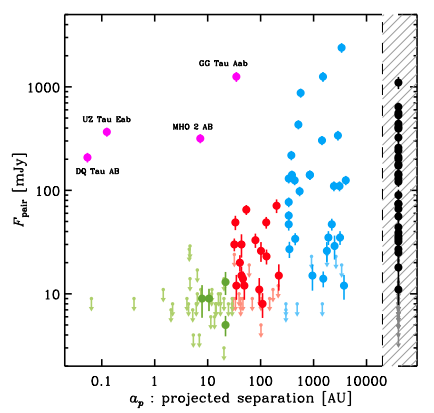
\includegraphics[width=0.5\linewidth]{harris2012_binary_brightnesses.png}}%
  \subcaptionbox{\citet{Akeson2019}}{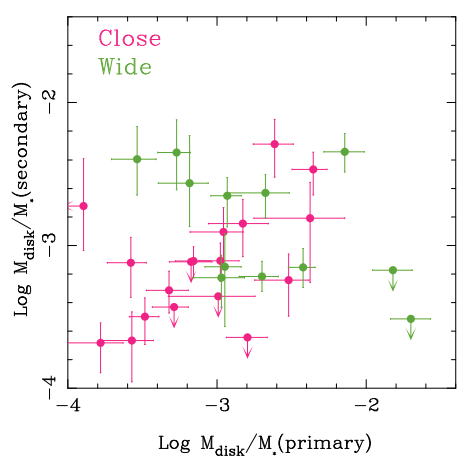
\includegraphics[width=0.5\linewidth]{akeson2019_binary_mass_ratios.png}}%
  \caption{Population trends from binary pairs in the Taurus star-forming region. ($a$): There is a clear upper limit on pair flux that is correlated to projected separation (green, red, and blue marks represent close, medium, and wide pairs). the presence of a circumbinary disk (magenta) yields an extra source of flux, and so pairs featuring such a disk do not follow the separation-limited flux pattern. ($b$): The mass of the disk around the secondary member of the binary in close systems (pink) is correlated to the mass of the primary, while in wide systems (green), the two are anti-correlated.}
  \label{fig:taurus_binaries}
\end{figure}

\begin{figure}[h]
  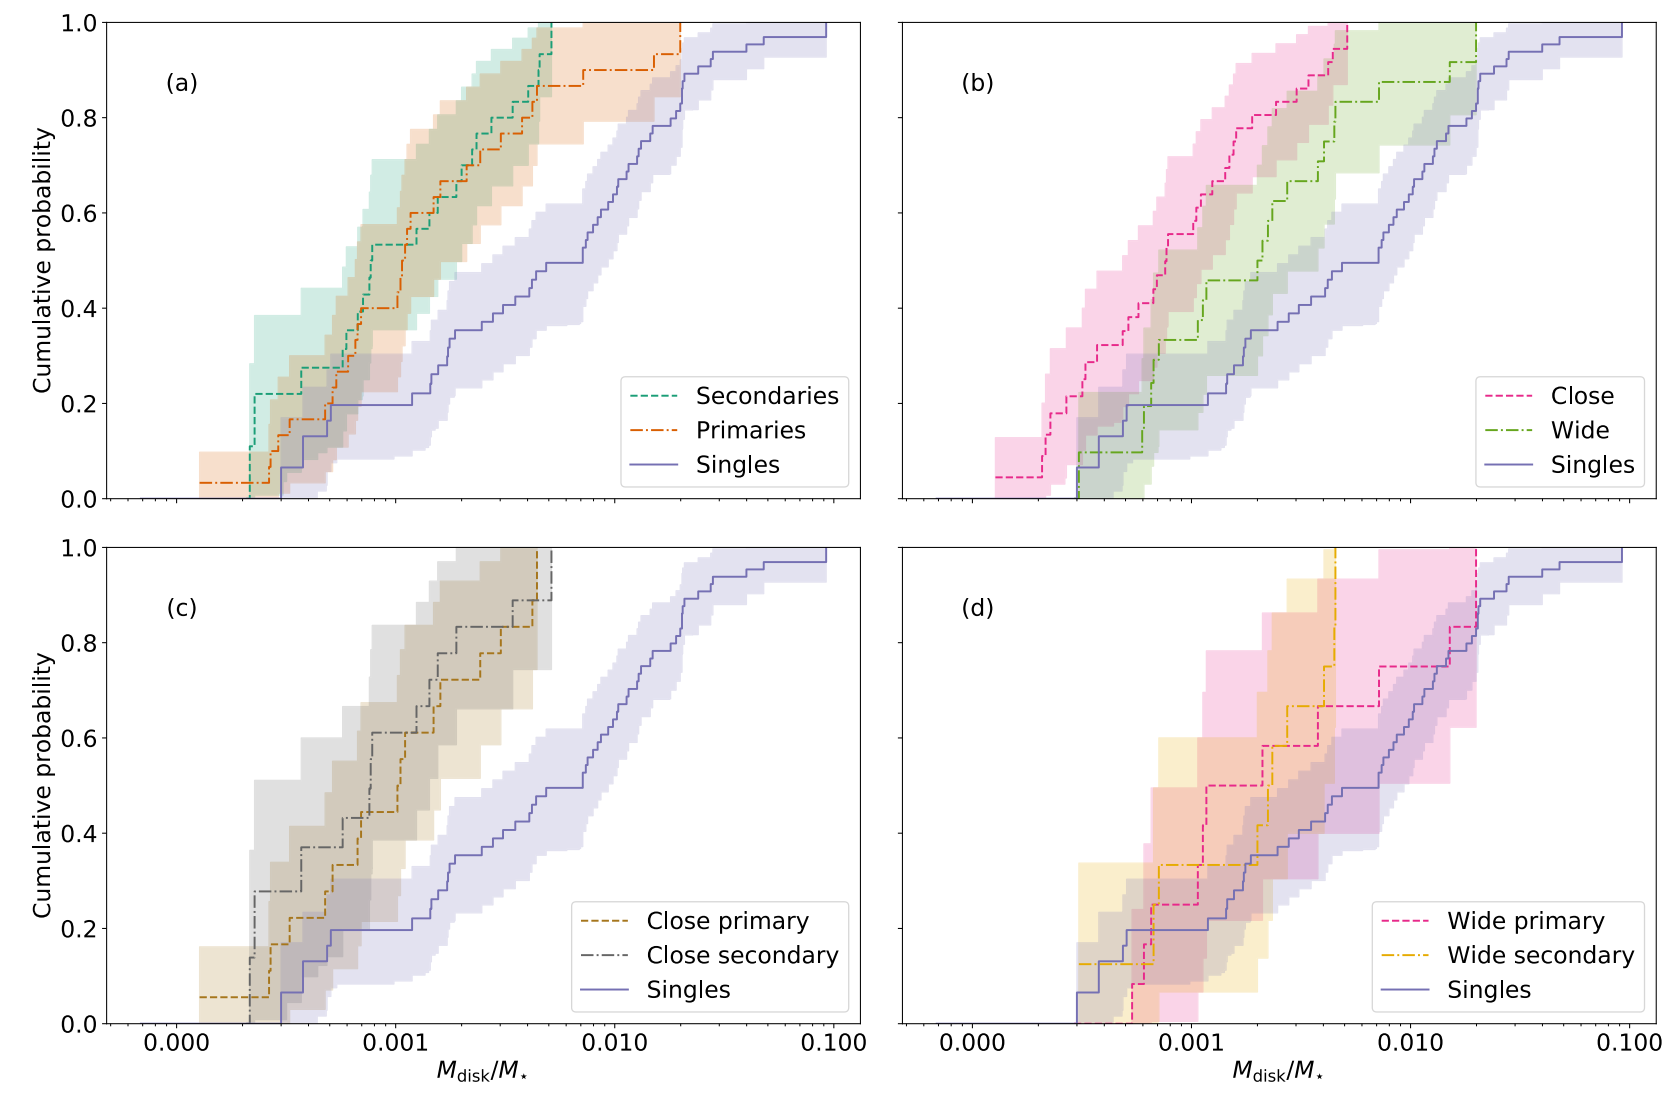
\includegraphics[width=\linewidth]{akeson2019_binary-disk-masses.png}%
  \caption{Cumulative probabilities of disk masses for different combinations of disks in binary pairs \citep{Akeson2019}. ($a$): Both disks in binary pairs are systematically less massive than single (isolated) disks although, as expected, the primary has more representation at the more massive end. ($b$): Close pairs are more significantly truncated than wide pairs, although wide pairs are still under-massive as well. ($c$) Close pairs do not preferentially truncate either disk; each has a sharp upper limit. ($d$): Primaries in wide pairs have nearly the same mass probability as single disks.}
  \label{fig:binary-disk-masses}
\end{figure}


% "For this sample of wide binaries, the secondary/primary disk mass ratio is not correlated with the secondary/primary stellar mass ratio. This suggests that for these binary systems, any environmental factors shared between the two components that could affect the initial disk mass and disk evolution are not the dominant factor in deter- mining the range of disk masses for a given stellar mass." (Akeson2014)

Disks in binary pairs have also been surveyed in the $\rho$ Ophiucus region. \citet{Akeson2014} studied 17 pairs with separations ranging from 101-990 au using ALMA, designed to measure the systems' masses. In it, they found no correlation between disk mass and stellar masses, matching the results from the studies of Taurus binaries above. \citet{Cox2017} followed with a survey targeting 63 total sources, comprised of 11 binaries, three triple systems, and 34 single sources; this also represented the first survey to characterize disk radii. In it, they, like \citet{Harris2012,Akeson2019}, found significantly lower fluxes from sources in binaries than isolated ones, and found that the disks' radii also exhibited systematic truncation. They note that this truncation is likely either due to tidal interactions between the disks or reflects a natural limit on the radii of disks in binaries, inherent to the disks' formation process, and that these decreased fluxes can be generally interpreted as being proportional to decreased masses. The authors also compared their sample to a $Spitzer$ survey of disks in Taurus \citep{Rebull2010}, and found that fluxes from disks in $\rho$ Ophiucus are typically dimmer than those in Taurus.


 \begin{figure}[h]
   \hspace*{\fill}%
   \subcaptionbox{}{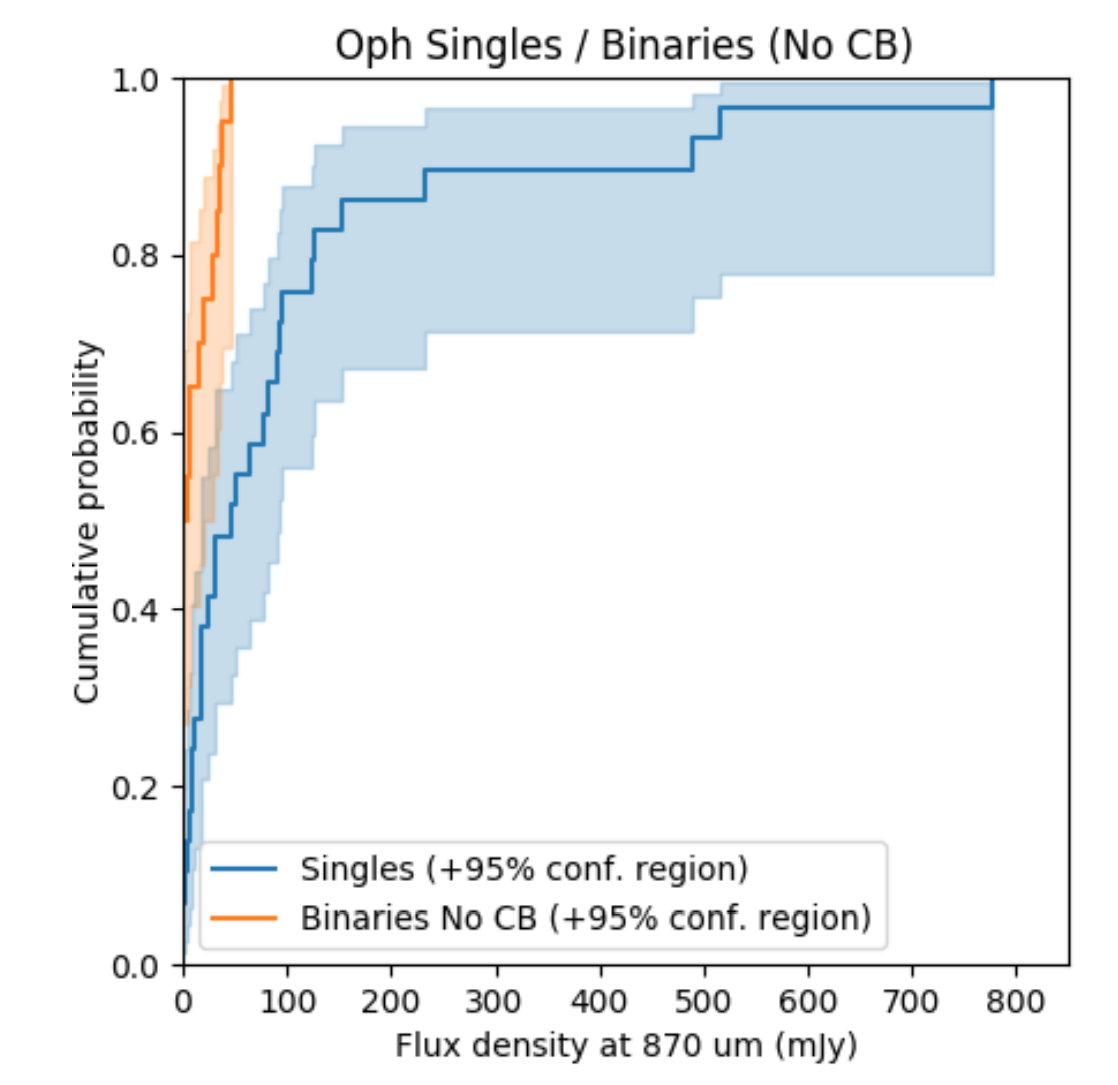
\includegraphics[width=0.5\linewidth]{cox17_rhoOph-singles-bins.png}}%
   \subcaptionbox{}{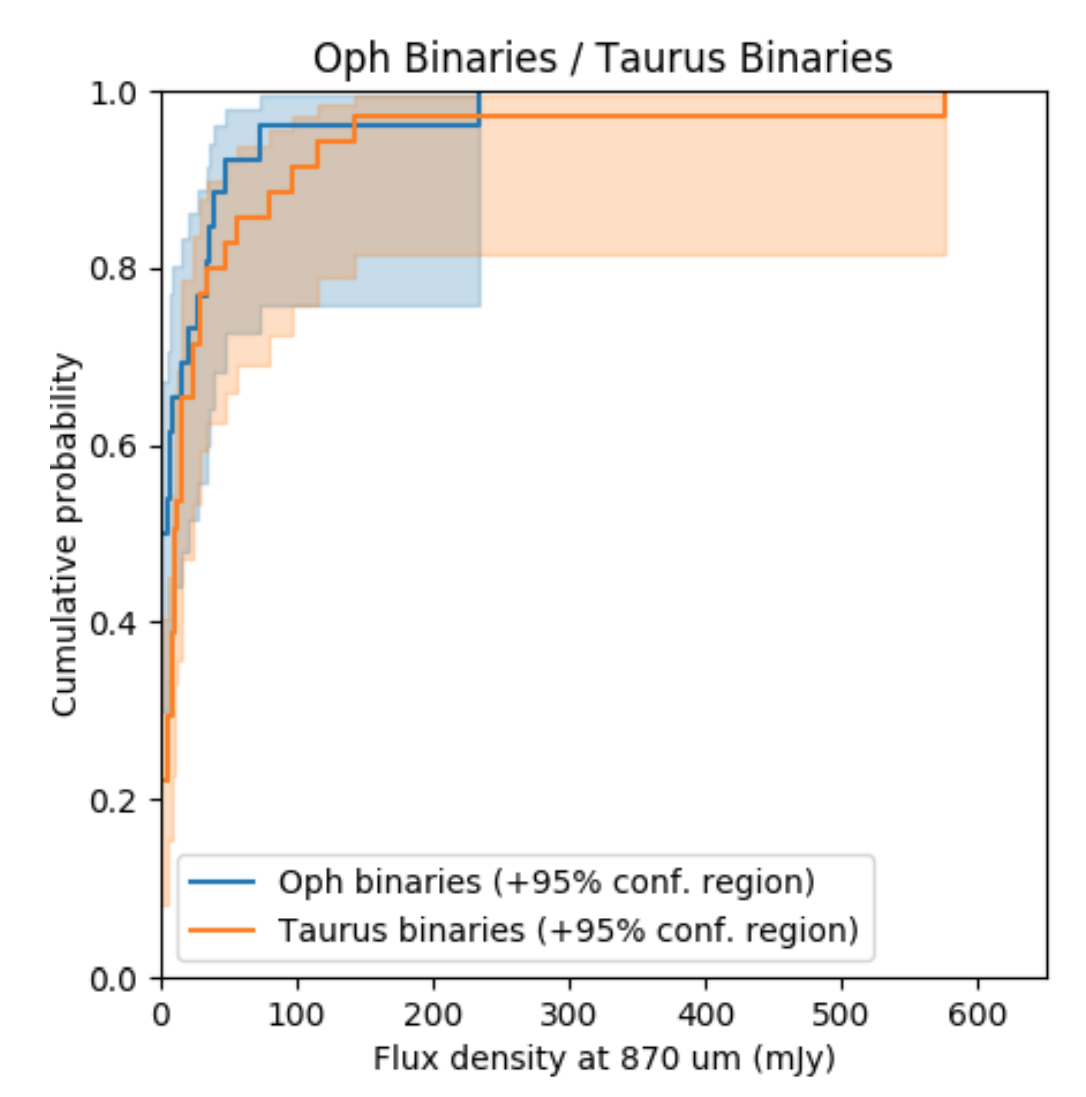
\includegraphics[width=0.5\linewidth]{cox17_taurus-rhhOph-bins.png}}%
   \hspace*{\fill}%
   \caption{\citet{Cox2017} showed that disks in binary systems (excluding circumbinary disks) in $\rho$ Ophiucus have systematically lower fluxes than both isolated disks in the region (\textit{left}) and disks in binaries in Taurus \citep[from][]{Rebull2012}.}
   \label{fig:rhoOph_binaries}
 \end{figure}



Comparing the present study's binary pair, however, immediately shows that its disks are neither faint nor small, neither in comparison to the disks in those surveys or to the disks in the survey that it was a part of. However, this is not really out of line from the morphological patterns presented in the surveys above since, at 428 au, the disks' projected separation is enough to put them beyond the reach of the most significant mass and radius truncations that closer binaries undergo.

% Implications of the disks' misaligned rotational axes. \citet{Lai2014} shows that it's pretty easy to make them misaligned.








\section{Chemical \& Temperature Structures}
% Chem modeling from Meredith
% Nomura, Henning, Ewine, Semmenov, Henning and Semminov Review on Disk Chem,

We now explore the chemical nature of protoplanetary disks. These disks have strong radial and vertical gradients in their temperatures, densities, and radiation fields, creating a wide range of environments for a wide range of chemistries. These chemistries can be broadly divided into inner- and outer-disk regimes, thanks to (typically) exponential radial temperature decay. Inner disk temps are high and thus best suited to IR observations, while outer disks are cold and thus better suited to sub-millimeter observations. Because our investigation is rooted in ALMA observations, we will only pursue an understanding of the outer disk here.

There are a number of ways to probe the chemical structures of a protoplanetary disk. Working with the basic building blocks of hydrogen, nitrogen, oxygen, and carbon and a wide diversity of temperature, density, turbulence, and radiation environments, disks are able to develop an array of molecules, each with its own characteristic formation conditions and emission signatures. Understanding disk chemistry is a process of knowing which of these signatures to look for and make sense of what they are telling us.


The first standard - the null hypothesis - for our fits to molecular abundance is the abundances found in molecular clouds, since that is the material from which these disks form. \citet{Aikawa1999} showed these to be X$_{\hco}$ = $9 \times 10^{-9}$ and X$_{HCN}$ = $2 \times 10^{-8}$; decreases from these values are to be somewhat expected in disks, as shown in \citet{REWORK GET REFERENCE}. However, since disks undergo complex chemical evolution, we would like to improve our predictions beyond just looking at ISM values. Modeling provides an appropriate context for observation in disk chemistry. Developing a parametric understanding of the chemical structure and evolution of protoplanetary disks guides our interpretation of data.


% Thanks to freeze-out and photodissociation, molecular abundances tend to be depleted by a factor of 5-100 in disks compared to the abundances found in the Taurus molecular cloud.

% \citet{Dutrey1997} first pointed out that molecular abundances were one to two orders of magnitude below molecular cloud levels in PPDs
\citet{Aikawa1997} were some of the first to apply time-evolving chemical networks to protoplanetary disks, describing the effects of cosmic rays in the outer disk and how they can change CO and N$_2$ - initially abundance molecules - into more complex organics, including HCN, through chemically active ions. \citet{Aikawa1999} expanded upon the work, modeling the evolution of molecular abundances in an accreting protoplanetary disk. They show that the timescale of this chemical evolution is dependent on the disk's ionization rate and the size distribution of the dust grains, increasing with lower ionization rates and/or larger grains and vice versa. As grains grow, HCN abundances are lowered by orders of magnitude, since they depend heavily on the grain surface recombination of \hco, which is significantly smaller in the case of larger grains. The authors show that abundances of HCN and \hco, initially set at $10^{-8}$ and $4 \times 10^{-9}$, increase dramatically (by around four magnitudes) with accretion over time.

\citet{AikawaHerbst1999} presented a two-dimensional ($r, z$) description of chemical evolution of a protoplanetary disk, defining temperature and density profiles and calculating the resulting interactions between the gas and dust, X-rays, and cosmic rays. They note here that, at significant differences from the midplane, a higher ionization rate can be seen due to X-rays, while the mid-plane is dominated by cosmic rays, and that certain abundances (including HCN) are enhanced by higher ionization rates. These simple, early models (whose most notable deficiency is the lack of physical evolution, a consequence of the limited computational power available at the time) yielded models that are surprisingly consistent with today's more complex models. This work was again built on by \citet{Aikawa2002}, in which they investigate the effects of a vertical temperature gradient. These efforts yielded approximately radially constant distributions of \hco and HCN and \hco presenting column densities about an order of magnitude above those of HCN.


\begin{figure}[h]
  \includegraphics[width=\linewidth]{Aikawa1999_chem_process_co.png}%
  \caption{The chemical process leading to the generation of \hco and HCN \citep{Aikawa1999}. We immediately see that the generation of \hco is directly dependent on CO, while that same \hco molecule can then combine with N to yield the disk's HCN.}
  \label{fig:disk_ionization}
\end{figure}

Disk chemistries are heavily influenced by high energy radiation introduced by the disk's host star and cosmic rays. \citet{Fogel2011} showed how UV radiation will selectively photodissociate certain molecules (Lyman $\alpha$ emission, for example, is strong in T Tauri stars and can have particularly strong effects on H$_2$O and HCN), and the selective photodissociation of CO by interstellar radiation. However, higher ionization rates typically lead to higher abundances of the molecules we are observing. For example, strong radiation fields (i.e. from neighboring massive stars) will have the effect of amplifying the disk's natural CO-based photo-chemistry (already driven by the host star) and increase the size of the disk's warm gas layer. Additionally, the disk's dust evolution can affect the gas \citep{Akimkin2013}, with grain growth and sedimentation leading to decreased UV shielding of the disks inner layers and pushing the disk's molecular layer closer to the midplane. As these larger grains and the molecular layer both settle to the midplane, molecular freezeout in the region is slowed, leading to heightened column densities for many species, including CO and HCN.

To study the effects of this ionization in anticipation of the opening of ALMA, \citet{Walsh2010} developed radial and vertical chemical models for an isolated protoplanetary disk around a T-Tauri star, watching molecular abundance distributions throughout the disk for molecules within ALMA's reach. They showed that log abundances in their models for \hco varied from $-8$ to $-12$, $-7$ to $-12$ for HCN, and $-4$ to $-9$ for CO. The authors then built on this model by adding functionality to model externally-driven UV and X-ray ionization \citep{Walsh2012} and applied it to the same disk system, this time with an O star nearby providing ionizing photons \citep{Walsh2013}. They then made the same molecular abundance distribution maps as before (see Fig.\ref{fig:walsh-abundance-profs}). The authors note that, in their model photoionized disk, \hco column density increases by a factor of 6.3 relative to the isolated disk, whereas HCN and CO column densities remain constant through ionization. They also note that the ionized disks have much higher gas temperatures, $\gg$ 50 K; this is consistent with the high temperatures that we see in our disks.


% This 6.3 increase would be useful if we had an estimation of what the \hco/HCN ratio would be in these two disks. They do have column density ratios in Walsh13; is it reasonable to say (I guess it would have to be in the case of optically thin emission) that col dens $\propto$ abundance? If that were the case then we'd be golden.

\begin{figure}[t]
  \hspace*{\fill}%
  \subcaptionbox{CO abundances}{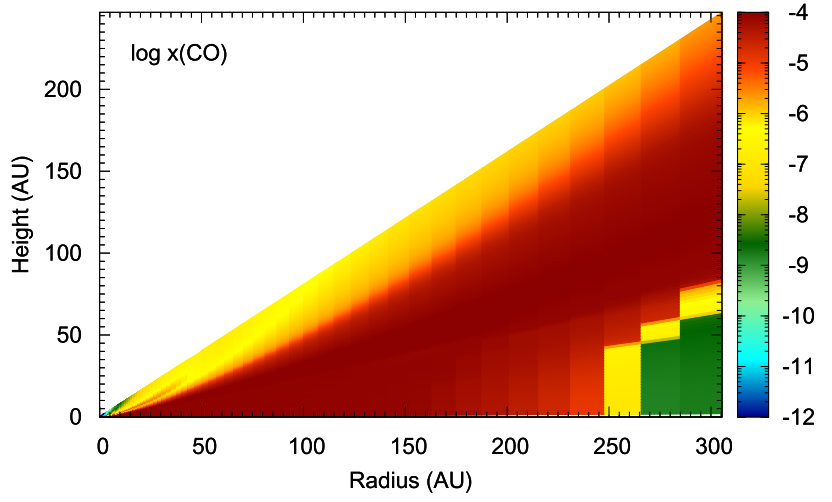
\includegraphics[width=0.33\linewidth]{walsh10_Xco.png}}%
  \subcaptionbox{\hco abundances}{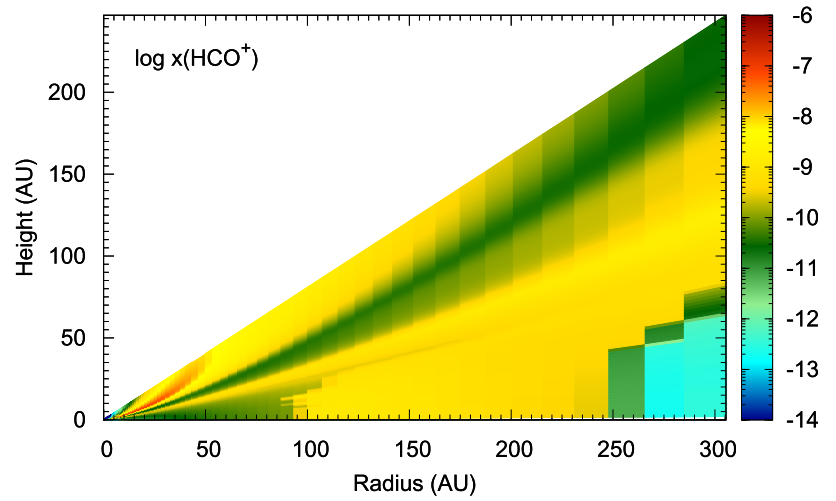
\includegraphics[width=0.33\linewidth]{walsh10_Xhco.png}}%
  \subcaptionbox{HCN abundances}{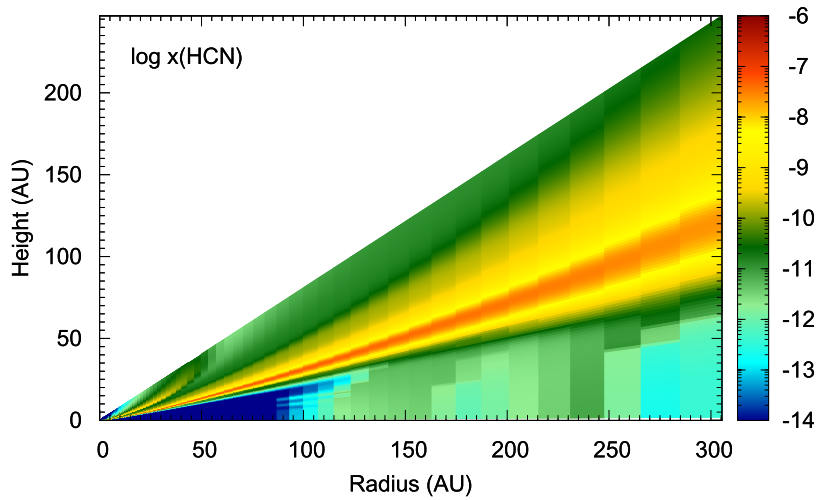
\includegraphics[width=0.33\linewidth]{walsh10_Xhcn.png}}\vfill%
  \subcaptionbox{CO abundances}{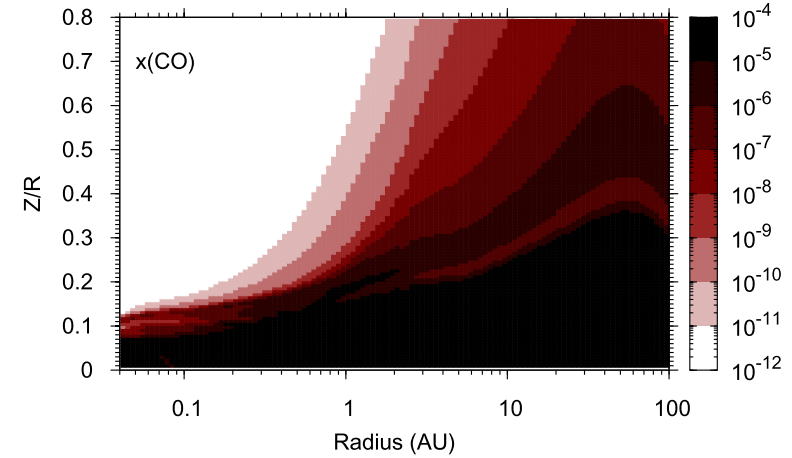
\includegraphics[width=0.33\linewidth]{walsh13_Xco.png}}%
  \subcaptionbox{\hco abundances}{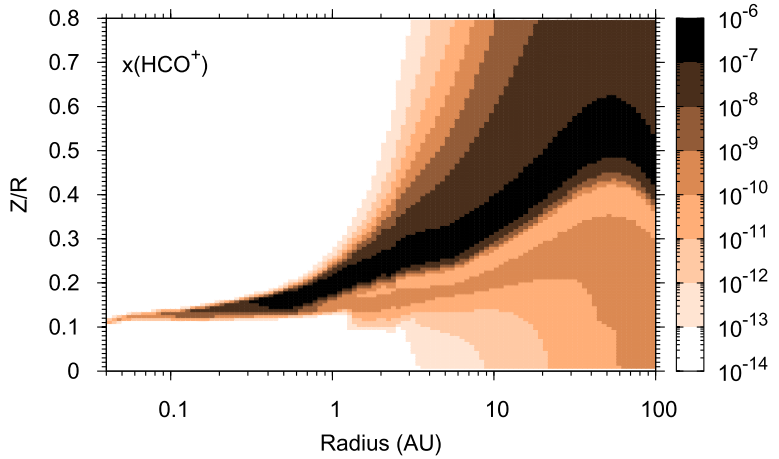
\includegraphics[width=0.33\linewidth]{walsh13_Xhco.png}}%
  \subcaptionbox{HCN abundances}{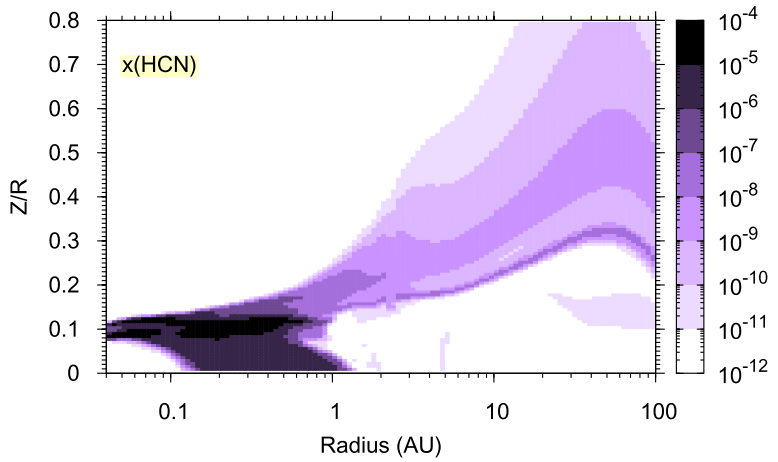
\includegraphics[width=0.33\linewidth]{walsh13_Xhcn.png}}%
  \hspace*{\fill}%
  \caption{Models showing radial and vertical distributions of CO, \hco, and HCN in a simulated disk around a T-Tauri star. The top row shows the profiles of isolated disks \citep{Walsh2010}, while the bottom row shows the profiles of disks being irradiated by a nearby O star \citep{Walsh2013}. Note that bottom row is on a log scale and only covers the inner 100 AU of the disk, while the top row is linearly scaled and shows a 300AU stretch. \textit{It seems like only having one of these sets of images would make more sense.}}
  \label{fig:walsh-abundance-profs}
\end{figure}


\citet{Cleeves2013,Cleeves2014} also sought an explanation of the radiation and ionization environment in these disks, developing models to compare the relative contributions of stellar UV, stellar X-rays, and cosmic rays (see Fig.\ref{fig:disk_ionization}). Their findings showed that \hco traces high cosmic ray (CR) rates, with its abundances dropping significantly with decreased CR contributions, thanks to its precursor, CO, freezing out in regions where CRs are the primary energy source but defient. They also note that \hco abundances can suffer from particularly high UV fluxes (from either Herbig host stars or high radiation environments), as CO can be photodissociated before having a chance to from \hco. These influences allow \hco to trace the warm molecular ionization regions where CO is present in the gas.


\begin{figure}[t]
  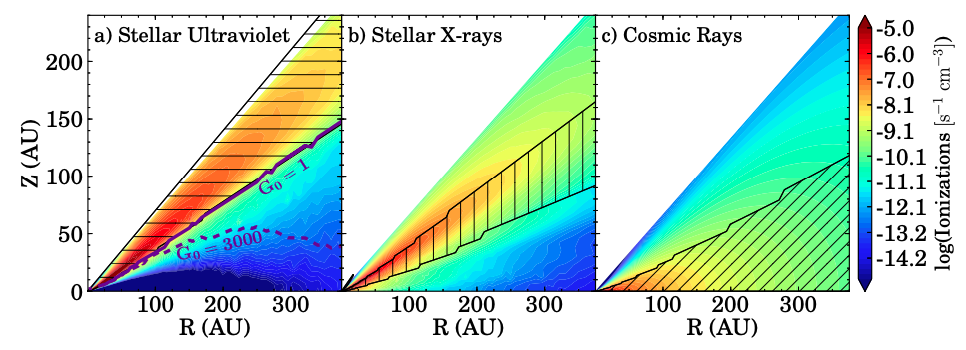
\includegraphics[width=\linewidth]{cleeves14_ionization_profiles.png}%
  \caption{Radiation contribution on a protoplanetary disk from stellar UV, stellar X-rays, and cosmic rays \citep{Cleeves2013}. The $G_0 = 1$ contour represents the effects from a host-only UV field (i.e. an isolated star), while the $G_0 = 3000$ contour represents the effects of a UV field made up of both the host as well as from the interstellar radiation field. \cite{Fatuzzo2008} showed 3000 to be a typical value for $G_0$ in clusters, thereby making it the more relevant model for our system.}
  \label{fig:disk_ionization}
\end{figure}

% From Fogel2011 -> AikawaHerbst1999: molecular cloud abundance vals: X$_\hco$ = 9e-9, X_$HCN$ = 2e-8.



% Some references:
% - Observations and modeling of gaseous protoplanetary disks (2008): https://iopscience.iop.org/article/10.1088/0031-8949/2008/T130/014011/pdf
% - CHEMICAL NETWORK REDUCTION IN PROTOPLANETARY DISKS: https://arxiv.org/pdf/1901.04888.pdf
%     - Fig 4 predicts low (-12) X_HCO+
% - The chemistry of disks around T Tauri and Herbig Ae/Be stars: https://arxiv.org/pdf/1803.09450.pdf
%     - Shouldn't see differences in HCN/HCO+/CS abundances between disks around TT and HA/HB stars
% - AN ALMA SURVEY OF DCN/H13CN AND DCO+/H13CO+ IN PROTOPLANETARY DISKS: https://arxiv.org/pdf/1701.01735.pdf
%     - Seems cool but idk what's going on
% - MULTIPLE PATHS OF DEUTERIUM FRACTIONATION IN PROTOPLANETARY DISKS: https://arxiv.org/pdf/1803.02498.pdf
%     - How DCO+ gets formed. Interesting, but not critically relevant
% - Physical and chemical structure of planet-forming disks probed by millimeter observations and modeling: https://arxiv.org/pdf/1402.3503.pdf
%     - A nice 2014 review, but not sure what to take away from it
% - The first multi-dimensional view of mass loss from externally FUV irradiated protoplanetary discs (2019): https://arxiv.org/pdf/1903.03644.pdf

% - Stellar disk destruction by dynamical interactions in the Orion Trapezium star cluster (2015): https://arxiv.org/pdf/1511.08900.pdf
% - External photoevaporation of protoplanetary discs in Cygnus OB2: linking discs to star formation dynamical history (2019): https://arxiv.org/pdf/1902.04586.pdf

% - Slideshow from Oberg: https://www.cfa.harvard.edu/sma/events/smaConf/posters/images/Oberg_SMA_archive.pdf
%   - p. 17: chemical depletion of CO


% Some more references:
% - Aikawa1999: https://iopscience.iop.org/article/10.1086/307400/pdf
% - Aikawa2002: https://arxiv.org/pdf/astro-ph/0202060.pdf
% - Semenov2011: Review of disk chem: https://arxiv.org/pdf/1107.4513.pdf
% - HenningSemenov2013: Bigger review of disk chem: https://pubs.acs.org/doi/pdf/10.1021/cr400128p
% - Akimkin2013: Modeling disk chem with dust: https://arxiv.org/pdf/1302.1403.pdf
% - Bergin+: Chem. Ev. of PPDs: http://www.ita.uni-heidelberg.de/research/klessen/internal/pp5/sec8-1.pdf
% - Harada2017: Grain growth effects on abundances: https://iopscience.iop.org/article/10.3847/1538-4357/aa602f/pdf
% - Dutrey2014: Phys. and Chem. Str. of PPDs: https://arxiv.org/pdf/1402.3503.pdf

% Not really sure what to do with all these. Create a full review of disk chemistry or just find the stuff relevant to my disks?


% Henning2013 (Table 1): HCN traces photochemistry, HCO+ traces ionization


On the temperature side, we expect in an idal disk to find $q=5$ (recalling that the radial temperature structure is generally assumed to go as $T(r) \propto r^{q}$). This can be found by recalling that the energy that a star emits decays as something. Such a structure invokes the assumption of a smooth, consistent distribution of emitting material, so variations from that value indicate variations in the structure. Studies of individal disks (in low-mass SFRs) have largely been in line with this prediction \citep[e.g. ][, whose values range from -0.22 to -0.7]{Dartois2003,Panic2008,Panic2010,Hughes2008,Qi2003,Qi2004,Isella2007,Rosenfeld2012,Flaherty2015,Flaherty2017,Zhang2017,Flaherty2018}. In their study of another ONC proplyd, \citet{Factor2017} found that their HCN emission traced a moderately-high structure of $q=-0.18$, but that their \hco line showed $q=0.17$.


The literature on disk temperatures is less well constrained, but it seems that higher ionization leads to higher temperatures.





% REWORL: Fix the Aikawa ref in the table, think bout whether it should be there. Also
\begin{table}[ht!]
  % \centering
  \begin{threeparttable}
    \caption{Disk Parameter List}
    \label{table:comparisons}
    \renewcommand{\arraystretch}{1.2}
    \begin{tabular}{l l l c c c }
      \toprule \toprule
      %\multirow{2}{*}{Parameter} & \multirow{2}{*}{Disk A}    & \multicolumn{2}{c}{Disk B} \\
      Reference                             & Source     & Line          & $q$ & log X$_\text{mol}$  & Atms. Temp (Measured Radius)\\
      \midrule %\midrule
      \multirow{3}{*}{This study}           & d253-1536a & \hco(4-3)      & $0.66$  & $-7.96$         & 151 (150 au) \\
                                            & d253-1536a & HCN(4-3)       & $0.72$  & $-7.62$         & 140 (150 au) \\
                                            & d253-1536a & CO(3-2)\tnote{a} & $0.40$  & $[-4]$        & 1 (150 au) \\
      \hline
      \multirow{3}{*}{\cite{Factor2017}}    & d216-0939  & \hco(4-3)      & $0.17$  & $-10.08$        & 190 (150 au) \\
                                            & d216-0939  & HCN(4-3)       & $-0.18$ & $-6.7$          & 19 (150 au) \\
                                            & d216-0939  & CO(3-2)        & $-0.33$ & $[-4]$          & 70 (150 au) \\
      % \hline
      % \multirow{3}{*}{\cite{Aikawa1999}}& Molecular Cloud  & \hco(4-3)      & $ [-]$  & $-10.08$        & 190 (150 au) \\
      %                                   & Molecular Cloud  & HCN(4-3)       & $ [-]$ & $-6.7$          & 19 (150 au) \\
      % \hline
      % \multirow{2}{*}{\citet{Flaherty2015}} & HD163296   & CO(3-2)        & $-0.22$ & $[-4]$          & 94 (150 au)  \\
      %                                       & HD163296   & CO(2-1)        & $-0.27$ & $[-4]$          & 79 (150 au) \\
      % \hline
      % \multirow{2}{*}{\citet{Dartois2003}}  & DM Tau     & $^{13}$CO(2-1) & $-0.30$   & $[-5.79]$       & 22 (100 au)  \\
      %                                       & DM Tau     & C$^{18}$O(2-1) & $-0.30$   & $[-5.79]$       & 35 (100 au) \\
      % \hline
      % \multirow{2}{*}{\citet{Chapillon2013}}& LkCa 15    & HCN(1-0)      & $-0.55$   & $[-]$          & 7   (300 au) \\
      %                                       & DM Tau     & HCN(1-0)       & $-0.0$   & $[-]$          & 36  (300 au)  \\
      % \multirow{2}{*}{\citet{Chapillon2018}}& CQ Tau     & CO(2-1)       & $-0.7$    & $[-]$          & 150 (100 au) \\
      %                                       & MWC 758    & CO(1-0)       & $-0.6$    & $[-]$          & 24  (100 au)  \\
      % \hline
      % \citet{Rosenfeld2012}\tnote{b}        & V4046 Sgr  & $^{12}$CO(2-1) & $-0.63$ & $[-4]$           & -  \\
      % \hline
      % % \citet{Dutrey2014}        & GG Tau A  & Continuum & $-1.1$ & NA          & 13.8  \\
      % % \hline
      % \citet{Flaherty2017}\tnote{c}         & HD163296   & DCO$^+$(3-2)   & $[-2.22]$ & $-10.79$      & [94]  \\
      % \hline
      % \citet{Zhang2017}                     & TW Hya     & $^{13}$C$^{18}$O(3-2), C$^{18}$O(3-2)  & $-0.47$ & -7.96 & 151  \\
      % \hline
      % \citet{Flaherty2018}\tnote{d}         & TW Hya     & CO(6-5, 3-2, 2-1) & $-0.46$ & $[-4]$       & 31  \\
      % Charlie Qi for this, and other mol. line stuff
      % French group (Dutrey, Dartois etc) (Simon et al (2010ish))
      % Panic 2008ish
      % Isella et al
      \bottomrule
    \end{tabular}
    \begin{tablenotes}\footnotesize
      \item[*] Values in [brackets] were fixed during fitting.
      \item[**] Since there is not a convention about whether a negative value of $q$ indicates a radially decreasing or increasing temperature structure (in other words, whether or not $q$ is implicitly negative), some of these values have the opposite sign of the value reported in their article. When this is the case, it indicates that, in that original paper, atmospheric temperature was defined such that T$_\text{atms} \propto r^{-q}$. In our work, and in all the values given here, it is the case that T$_{atms} \propto r^{q}$, meaning that a negative value of $q$ leads to temperature decreasing with radius.
      \item[a] This result is being presented for completeness (and to allow for the chance that something changes dramatically in coming runs REWORK), but since its T$_{atms}$ clearly got stuck, it is not a useful result for comparison and will not be discussed.
      \item[b] \cite{Rosenfeld2012} didn't fit for tatms
      \item[c] In \citet{Flaherty2017}, they fit three rings, and consequently have three slightly different values for each parameter. The values reported here are for their middle ring, although the three do not vary significantly from one another. Additionally, T$_{atms}$ and $q$ were fixed at values found for CO(3-2) in \citet{Flaherty2015}, and only X$_\text{mol}$ was fit for.
      \item[d] \citet{Flaherty2018} developed several models, with different morphological structures. The results presented here are drawn from their simplest (fiducial) model.
    \end{tablenotes}
  \end{threeparttable}
\end{table}
% TO ADD:
% Dutrey 2014: Disks in CG Tau: https://www.nature.com/articles/nature13822#abstract


Table \ref{table:comparisons} presents molecular abundances and temperature structure parameters for disks from a selection of studies. While the list is not comprehensive \citep[see ][for more example]{Panic2008,Panic2010,Hughes2008,Qi2003,Qi2004,Isella2007}), its members were selected to highlight features from a diversity of emission lines. The most immediately relevant of these is the work by \citet{Factor2017}, the only other study to do forward-modeling of emission using a ray tracing code. In it, they characterize another ONC proplyd from the same survey as our binary, and thus represents the only other study to model a disk that is also in a high-mass star forming region. The other studies listed are focus on disks in low-mass regions. We may compare our temperature profiles and abundance to these other systems and look for variations from typical values.

There are several points of note here. Save for the CO line, which shows nonphysical temperatures, our atmospheric temperatures are notably higher than those found in the other studies. Additionally, our temperature structures for both \hco and HCN are solidly positive, reflecting a structure that increases with radius. As with the atmospheric temperature, this is contrasted by all other results, which have moderately negative values, save again for that of the \citet{Factor2017} \hco line, which is also positive but less so than in our fits. Our positive values stand somewhat in contrast to the $q$ value of $-0.5_{-0.1}^{0.2}$ predicted by \citet{Dartois2003} for a geometrically flat, optically thin disk. \citet{Schwarz2016} note that a flatter, non-negative structure is to be expected when observing emission that originates from layers just above freeze out temperature in the disk.

% It is possible that these atypical findings are a result of the MCMC fitting algorithm  trying to fit the
% REWORK on "stand somewhat in contrast...": "I’d remove the “somewhat,” and add some information about why you expect the decreasing temperature structure.  Then you could talk about some of the methodology that is likely to be influencing your result: spatially unresolved systems, assumptions about freeze-out and photodissociation that might lead the algorithm to artificially require increased temperatures just to have any molecular emission at large radii, etc."













\section{How d253-1536 Stacks Up}
% you can do a pretty detailed comparison of your disk vs. Sam’s disk (in the table, yes, but also discussed in words in the text) and then you can compare with disks from low-mass SF regions as well (again, you’ve got a lot of the seeds of that discussion here).

% REWORK: "In terms of content, this is a great start, but how exhaustive is it?  I think you need to specify exactly what you’re doing with this table, and how you decided which disks to compare with and which ones not to.  The French group (Guilloteau, Dutrey, and others) would be very upset that you didn’t include any of their work, for example!  I really like the idea behind this table, but I think you need to go big or go home — make sure you’re specific about what is included in the table, and then make sure you are thorough about including all the relevant studies."

With a theoretical structure now in place, we can now compare our results to that literature, as well as other specific disks.

blah blah







% ABUNDANCES


\citet{Factor2017} found \hco abundances in line with these predictions, but a significant excess of HCN, consistent with high ionization rates REWORK AND SOMETHING ELSE?

Our fits show disk A having a notable excess in both lines and more typical abundances in disk B.

That each disk's abundances are so different from one another is something of a surprise. Both disks have similar ratios of the two emitting molecules: disk A's \hco/HCN ratio of log abundances is 1.09, while disk B's is 0.95, becoming 1.21 for disk A and unity for disk B if the disk B radius cut is made.












We see in the HCN channel maps an area of significant flux coming from between disks around $ v = 9-11$ \kms. This may be region where the two disks are interacting, a possibility that our model does not take into account. The feature is less clearly present in \hco and invisible in CO, likely overrun by cloud contamination. \citet{Smith2005} note that disk A "exhibits distortions that we attribute to tidal interactions with the companion star" (before they knew that there is a second disk).













\section{Implications}
% - The thing that’s really missing from the discussion is a conversation about what this all means.  *Why* might the similarities/differences between your disk and Sam’s, or your disk and the ones in low-mass SFRs exist?  I think you will be able to write it a lot better once you have expanded your reading beyond just Catherine Walsh’s modeling.  What factors do the modelers predict should affect the chemistry of these disks?  How are these factors related to environment?  To what extent might they be influenced by binarity?  

% MASS DISCUSSION
With this context, how do now we make sense of our current observations and fits? Our results show a wide (428 au separation) binary pair of stars with disks that are massive\footnote{Although this mass is, of course, still handicapped by the assumptions about gas/dust ratios} and radially large (both compared to other disks in the ONC and disks in binaries in Taurus and $\rho$ Ophiucus). The two disks have appreciably different chemistries, and are physically interacting, as shown by the HCN residuals.


\citet{Andrews2013} showed that the masses of disks in Taurus are linearly correlated with the mass of their host stars, going as M$_\text{disk} \approx 0.4$\% M$_\star$ and ranging by up to a factor of 40. Our disks have masses approximately equal to 2\% and 7\% of their host stars for disk A and B, respectively, which is consistent with their linear fit and the associated uncertainty. There is also sufficient uncertainty in the measurement of these disks' masses - from the 100:1 gas/dust ratio and dust temperatures assumed in the mass calculation - that these values lack the precision necessary to





% TEMPS
Regarding the disks' differing chemistries and high temperatures, several explanations are possible. The most obvious explanation is that, since the disks are hosted by stars of very different masses and spectral types (disk A's host is a 3.5 M$_\odot$ F or G star, and disk B is hosted by an accreting 0.4 M$_\odot$ M2.5 star), theory predicts that they have different chemistries. Since the more massive star would be a stronger emitter of UV radiation, and since, as described above, the resulting ionization leads to expansion of the warm molecular layer and significant increases in the abundances of these molecules as well as heightened disk temperatures. As discussed above, it is predicted that high incident UV fluxes should lead to the increased production of \hco and, in turn, HCN, and that these abundances reflect that.

% REWORK: Would be really nice to figure out the relationship between HCO and HCN. What does HCN trace?

Another known way to increase the abundances of these species is by increasing the dust mass around them. A simple calculation of the dust mass-to-radius ratio for these disks reveals that this pseudo-measure of density is not the same for the two disks (maybe do the error propogation thing here?).
% Andrews, Tripathi, maybe someone else on mass/radius dust ratios
% 78/335 = 0.23
% 30/145 = 0.2


% REWORK: "Yes, very speculative.  How about mentioning some other possibilities?  For example, if the central stars are different spectral types, that could affect the photochemistry, or different initial disk masses/optical depths could affect how the disks evolve, or planets… try thinking of some more possibilities, and dig into the literature to find some references (they are out there!)"
A less probable but still fascinating possibility is that these disks did not form together. \citet{Williams2014} posit that wide binaries (systems with separations $\geq$ 300 au), such as this one, do not form in the same initial cloud structures. If this were the case, then it might be reasonable to expect each disk to reflect different chemical histories from the regions of the cluster in which each formed. However, binary capture is rare, as a third star is required for this proces to create a bound pair \citep[e.g. ][]}{Mansbach1970}, and it is unclear whether the local stellar environment shows history of such an event. It is also unclear how the binary's stellar mass ratio - around 9:1 - would affect the capture process.

% REWORK: Re the footnote: "Hm, I’m not sure either, but I would take a look at Robert Harris’s PhD thesis papers on binaries with the SMA as a starting point — check his intro and discussion for relevant references.  Could also check the more recent Akeson/Jensen papers on binaries with ALMA for some relevant intro/discussion material.  Would be good to expand upon this point in the discussion."

Density fluctuations could also contribute to variations in the disks' chemistries as well, be it in the form of embedded planets or turbulence. Since we do not fully resolve disk A and do not resolve disk B, this becomes a particularly speculative step, but \citet{Miotello2016} propose that disks could preferentially chemically depleted through molecules being locked up in larger bodies that are invisible in the radio.
% REWORK: what is the effect of a planet on disk chemistry?


% pabst2019_onc_ionization


Regardless of what the primary driver of this chemical asymmetry between the two disks, the radiation environment in which these disks exist is a fascinating one, thanks to the unique combination of a relatively high-mass star (d253-1536a), an heavily-accreting M-star (d253-1536b), and, even though they are far from the Trapezium cluster, \citet{Pabst2019} recently showed that marginal ionization from Trapezium is still present well past M43 (see Fig.\ref{pabst2019_onc_ionization}).




\begin{figure}[h]
  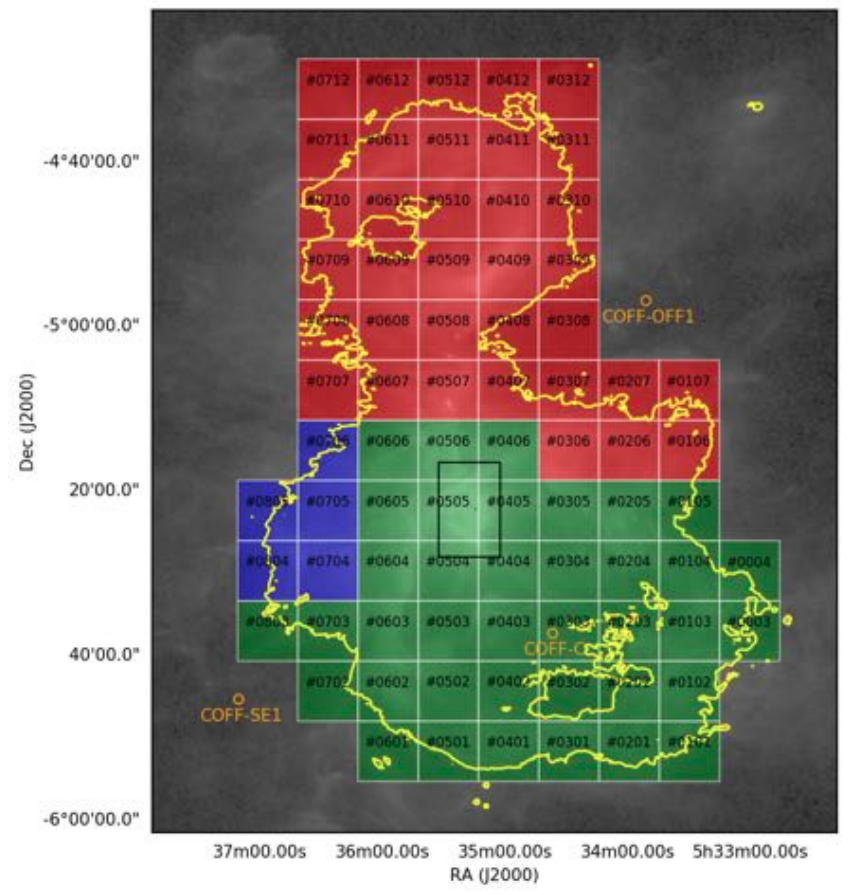
\includegraphics[width=\linewidth]{pabst2019_onc_ionization.png}%
  \caption{blah blah}
  \label{fig:pabst2019_onc_ionization}
\end{figure}








% The End
